%%%%%%%%%%%%%%%%%%%%%%%%%%%%%%%%%%%%%%%%%%%%%%%%%%%%%%%%%%%%%%%%%%%%%%%%%%%%%%%%%%%
%% This project aims to create the UFC template for presentation.                %%
%% author: Maurício Moreira Neto - Doctoral student in Computer Science (MDCC)   %%
%% contacts:                                                                     %%
%%    e-mail: maumneto@ufc.br                                                    %%
%%    linktree: https://linktr.ee/maumneto                                       %%
%%%%%%%%%%%%%%%%%%%%%%%%%%%%%%%%%%%%%%%%%%%%%%%%%%%%%%%%%%%%%%%%%%%%%%%%%%%%%%%%%%%
\documentclass{libs/ufc_format}
% Inserting the preamble file with the packages
%%%%%%%%%%%%%%%%%%%%%%%%%%%%%%%%%%%%%%%%%%%%%%%%%%%%%%%%%%%%%%%%%%%%%
%% This file contains the packages that can be used in the beamer. %%
%%%%%%%%%%%%%%%%%%%%%%%%%%%%%%%%%%%%%%%%%%%%%%%%%%%%%%%%%%%%%%%%%%%%%
% Package to fonts family
\usepackage[T1]{fontenc}
% Package to accentuation
\usepackage[utf8]{inputenc}
% Package to Portuguese language
\usepackage[brazil]{babel}
% Package to Figures
\usepackage{graphicx}
% Package to the colors
\usepackage{color}
% Package to the colors
\usepackage{xcolor}
% Packages to math symbols and expressions
\usepackage{amsfonts, amssymb, amsmath}
% Package to multiple lines and columns in table
\usepackage{multirow, array} 
% Package to create pseudo-code
% For more detail of this package: http://linorg.usp.br/CTAN/macros/latex/contrib/algorithm2e/doc/algorithm2e.pdf
\usepackage{algorithm2e}
% Package to insert code
\usepackage{listings} 
\usepackage{keyval}
% Package to justify text
\usepackage[document]{ragged2e}
% Package to manage the bibliography
\usepackage[backend=biber, style=numeric, sorting=none]{biblatex}
% Package to facilities quotations
\usepackage{csquotes}
% Package to use multicols
\usepackage{multicol}

% Packages added by me
\usepackage{url}
\usepackage{tikz}
%\usepackage{multimedia}
%\usepackage{media9}[playbutton=plain, windowed=1280x720]
% Inserting the references file
\bibliography{references.bib}
\renewcommand*{\bibfont}{\scriptsize}

% Title
\title[Introdução a IA]{\huge\textbf{Introdução à Inteligência Artificial}}
% Subtitle
\subtitle{Parte 2}
% Author of the presentation
\author{Evandro J.R. Silva}
% Institute's Name
\institute[Estácio Teresina]{
    % email for contact
    \normalsize{\email{ejrs.profissional@gmail.com}}
    \newline
    % Department Name
    %\department{Bacharelado em Ciência da Computação}
    \newline
    % university name
    %\ufc
    \estaciothe
}
% date of the presentation
\date{30 e 31 de Janeiro}


%%%%%%%%%%%%%%%%%%%%%%%%%%%%%%%%%%%%%%%%%%%%%%%%%%%%%%%%%%%%%%%%%%%%%%%%%%%%%%%%%%
%% Start Document of the Presentation                                           %%               
%%%%%%%%%%%%%%%%%%%%%%%%%%%%%%%%%%%%%%%%%%%%%%%%%%%%%%%%%%%%%%%%%%%%%%%%%%%%%%%%%%
\begin{document}
% insert the code style
%%%%%%%%%%%%%%%%%%%%%%%%%%%%%%%%%%%%%%%%%%%%%%%%%%%%%%%%%%%%%%%%%%%%%%%%%%%%%%%%%%%
%% This file contains the style of the codes show in slides.                     %%
%% The package used is listings, but it possible to used others.                 %%
%%%%%%%%%%%%%%%%%%%%%%%%%%%%%%%%%%%%%%%%%%%%%%%%%%%%%%%%%%%%%%%%%%%%%%%%%%%%%%%%%%%

% color used in the code style
\definecolor{codegreen}{rgb}{0,0.6,0}
\definecolor{codegray}{rgb}{0.5,0.5,0.5}
\definecolor{codepurple}{rgb}{0.58,0,0.82}
\definecolor{codebackground}{rgb}{0.95,0.95,0.92}

% style of the code!
\lstdefinestyle{codestyle}{
    backgroundcolor=\color{codebackground},   
    commentstyle=\color{codegreen},
    keywordstyle=\color{magenta},
    numberstyle=\tiny\color{codegray},
    stringstyle=\color{codepurple},
    basicstyle=\ttfamily\footnotesize,
    frame=single,
    breakatwhitespace=false,         
    breaklines=true,                 
    captionpos=b,                    
    keepspaces=true,                 
    numbers=left,                    
    numbersep=5pt,                  
    showspaces=false,                
    showstringspaces=false,
    showtabs=false,                  
    tabsize=2,
    title=\lstname 
}

\lstset{style=codestyle}


%% ---------------------------------------------------------------------------
% First frame (with tile, subtitle, ...)
\begin{frame}{}
    \maketitle
\end{frame}

%% ---------------------------------------------------------------------------
% Second frame
\begin{frame}{Sumário}
    \begin{multicols}{2}
        \tableofcontents
    \end{multicols}
\end{frame}

%=============================================================================
% SECTION 1
%=============================================================================
\section{Agentes Inteligentes}

\begin{frame}{}
    \centering
    \Large
    Agentes Inteligentes
\end{frame}

\begin{frame}{Agentes Inteligentes}
    \begin{itemize}
        \justifying
        \item O que seria um agente?
            \begin{itemize}
                \justifying
                \item Tudo o que pode ser considerado capaz de perceber seu \textbf{ambiente} por meio de \textbf{sensores} e de agir sobre esse ambiente por intermédio de \textbf{atuadores}.
            \end{itemize}
        \item<2-> Outros termos importantes:
            \begin{itemize}
                \justifying
                \item<2-> \textbf{Percepção}: entradas perceptivas do agente em um dado instante.
                \item<3-> \textbf{Sequência de percepções}: a história completa de tudo o que o agente já percebeu.
                \item<4-> \textbf{Função do agente}: o mapeamento (em termos matemáticos) de qualquer sequência de percepções específica para uma ação.
                \item<5> \textbf{Programa do agente}: a implementação ``concreta'' da função do agente.
            \end{itemize}
    \end{itemize}
\end{frame}

\begin{frame}{Agentes Inteligentes}
    \centering
    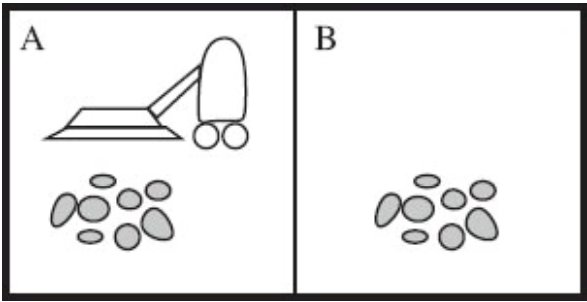
\includegraphics[width=0.45\textwidth]{figuras/figura03}
    \uncover<2>{
    \begin{table}[]
        %\footnotesize
        \scriptsize
        \begin{tabular}{|l|r|}
            \hline
            \textbf{Sequência de percepções} & \textbf{Ação}\\
            \hline
            [A, Limpo]  &   \\\relax %the \relax is to let [] in the next line
            [A, Sujo]   &   \\\relax
            [B, Limpo]  &   \\\relax
            [B, Sujo]   &   Direita\\\relax
            [A, Limpo], [A, Limpo]  &   Aspirar\\\relax
            [A, Limpo], [A, Sujo]   &   Esquerda\\\relax
            .           &   Aspirar\\
            .           &   Direita\\
            .           &   Aspirar\\\relax
            [A, Limpo], [A, Limpo], [A, Limpo]  &   \\\relax
            [A, Limpo], [A, Limpo], [A, Sujo]   &   Direita\\
            .           &   Aspirar\\
            .           &   \\
            .           &   \\
            \hline
        \end{tabular}
        \caption{Função do agente}
        \label{tab:my_label}
    \end{table}
    }
\end{frame}

\begin{frame}{Agentes Inteligentes}
    \begin{itemize}
        \justifying
        \item Como preencher a tabela de Função do agente da melhor forma?
        \item<2-> Como fazer com o agente seja, de fato, \textit{inteligente}?
        \item<3-> Se ele fizer tudo de forma \textit{correta}.
        \item<3-> Como definir se o agente fez algo da forma correta?
        \item<4> Através de uma medida de desempenho.
    \end{itemize}
\end{frame}

%-----------------------------------------------------------------------------
% SUBSECTION 1.1
%-----------------------------------------------------------------------------
\subsection{Medida de Desempenho}

\begin{frame}{Medida de Desempenho}
    \begin{itemize}
        \justifying
        \item Não há uma medida de desempenho fixa para todas as tarefas e agentes.
        \item Normalmente, um projetista vai desenvolver uma adequada às circunstâncias.
        \item Aparentemente é fácil...
            \begin{itemize}
                \justifying
                \item<2-> Vamos propor a seguinte medida de desempenho para o agente aspirador de pó: a quantidade de sujeira aspirada em um único turno.
                \item<2> É uma boa medida de desempenho?
                \item<3> E se o o robô começa a limpar, e depois suja de propósito, limpa, e suja, e limpa ... O desempenho para a tarefa dele aumenta significativamente!
                \item<3> Como resolver?
                \item<4> Como regra geral, é melhor projetar medidas de desempenho de acordo com o resultado realmente desejado no ambiente, em vez de criá-las de acordo com o comportamento esperado do agente.
                \item<4> Queremos racionalidade!
            \end{itemize}
    \end{itemize}
\end{frame}

%- - - - - - - - - - - - - - - - - - - - - - - - - - - - - - - - - - - - - - -
% SUBSUBSECTION 1.1.1
%- - - - - - - - - - - - - - - - - - - - - - - - - - - - - - - - - - - - - - -
\subsubsection{Racionalidade}

\begin{frame}{Racionalidade}
    \begin{itemize}
        \justifying
        \item<1> A definição do que é racional em qualquer instante depende de quatro fatores:
            \begin{itemize}
                \justifying
                \item A medida de desempenho que define o critério de sucesso.
                \item O conhecimento prévio que o agente tem do ambiente.
                \item As ações que o agente pode executar.
                \item A sequência de percepções do agente até o momento.
            \end{itemize}
    \end{itemize}
    \uncover<2>{
        \begin{block}{Agente Racional}
            \justifying
            Para cada sequência de percepções possível, um agente racional deve selecionar uma ação que se espera venha a maximizar sua medida de desempenho, dada a evidência fornecida pela sequência de percepções e por qualquer conhecimento interno do agente.
        \end{block}
    }
\end{frame}

\begin{frame}{Racionalidade}
    \centering
    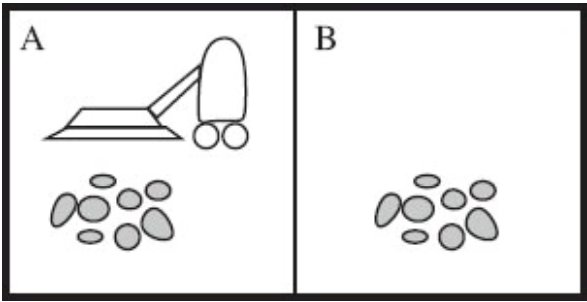
\includegraphics[width=0.45\textwidth]{figuras/figura03}
    \begin{enumerate}
        \justifying
        \item O robô recebe 01 ponto para cada quadrado limpo.
        \item O robô percebe em que quadrado está e qual o estado do quadrado.
        \item As únicas ações possíveis são \textit{Esquerda}, \textit{Direita} e \textit{Aspirar}.
        \item Quadrados limpos permanecem limpos.
    \end{enumerate}
    \justifying
    Em qual das seguintes situações poderíamos dizer que temos um agente racional?
        \begin{enumerate}[(a)]
            \item \textit{Direita} $\rightarrow$ \textit{Esquerda} $\rightarrow$ \textit{Direita} $\rightarrow$ ...
            \item \textit{Aspira} $\rightarrow$ \textit{Direita} $\rightarrow$ \textit{Aspira}.
        \end{enumerate}
\end{frame}

\begin{frame}{Racionalidade}
    \begin{itemize}
        \justifying
        \item O exemplo que vimos até então é sobre um mundo muito simples e estático.
        \item Um agente inteligente deve ser capaz de realizar sua tarefa independente do ambiente (levando-se em consideração que os projetistas sabem como \alert{classificar} o ambiente).
    \end{itemize}
\end{frame}

%-----------------------------------------------------------------------------
% SUBSECTION 1.2
%-----------------------------------------------------------------------------
\subsection{A Natureza dos Ambientes}

\begin{frame}{A Natureza dos Ambientes}
    \centering
    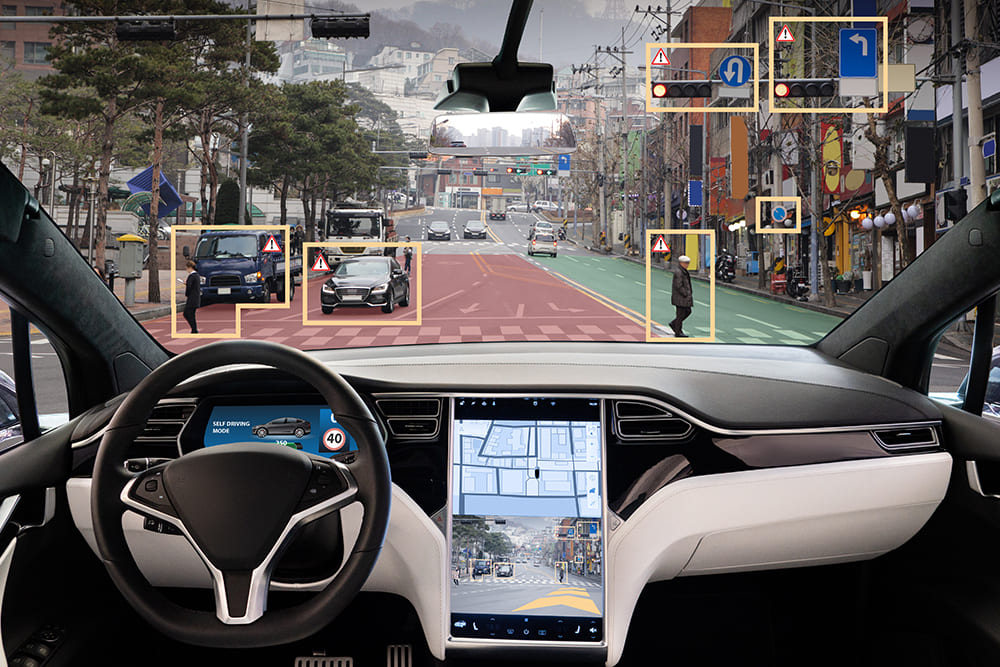
\includegraphics[width=\textwidth]{figuras/tesla.jpg}
\end{frame}

\begin{frame}{A Natureza dos Ambientes}
    \begin{table}[]
        \centering
        \footnotesize
        \setlength{\tabcolsep}{5pt}
        \begin{tabular}{p{0.15\textwidth}p{0.15\textwidth}p{0.15\textwidth}p{0.15\textwidth}p{0.15\textwidth}}
        \hline
        \textbf{Agente} & \textbf{Medida de Desempenho} & \textbf{Ambiente} & \textbf{Atuadores} & \textbf{Sensores}\\
        \hline
        \uncover<2->{Piloto Automático} & \uncover<3->{Viagem segura, rápida, dentro da lei, confortável, maximizar os lucros} & \uncover<4->{Estrada, tráfego, pedestres e clientes} & \uncover<5->{Direção, acelerador, freio, sinal, buzina} & \uncover<6->{Câmeras, sonar, velocímetro, GPS, etc.}\\
        \hline
        \end{tabular}
        \caption{Agente e Ambiente}
        \label{tab:my_label}
    \end{table}
\end{frame}

\begin{frame}{A Natureza dos Ambientes}
    \begin{itemize}
        \item Propriedades de ambientes
            \begin{itemize}
                \justifying
                \item \textbf{Completamente observável} \textit{vs.} \textbf{Parcialmente observável}
                    \begin{itemize}
                        \justifying
                        \item<1> Um ambiente de tarefa é de fato completamente observável se os sensores detectam todos os aspectos que \textit{são relevantes} para a escolha da ação.
                        \item<1> Se o agente não tiver sensores, o ambiente será \textbf{inobservável}.
                    \end{itemize}
                \item<2-> \textbf{Agente único} \textit{vs.} \textbf{Multiagente}
                    \begin{itemize}
                        \justifying
                        \item<2> Havendo dois ou mais agentes, o ambiente pode se tornar \textbf{competitivo} ou \textbf{cooperativo}.
                    \end{itemize}
                \item<3-> \textbf{Determinístico} \textit{vs.} \textbf{Estocástico}
                    \begin{itemize}
                        \justifying
                        \item<3> Se o próximo estado do ambiente é completamente determinado pelo estado atual e pela ação executada pelo agente, dizemos que o ambiente é determinístico; caso contrário, ele é estocástico.
                    \end{itemize}
                \item<4> \textbf{Episódico} \textit{vs.} \textbf{Sequencial}
                    \begin{itemize}
                        \justifying
                        \item<4> Em um ambiente de tarefa episódico, a experiência do agente é dividida em episódios atômicos. Em cada episódio, o agente recebe uma percepção e em seguida executa uma única ação.
                        \item<4> Por outro lado, em ambientes sequenciais, a decisão atual poderia afetar todas as decisões futuras.
                    \end{itemize}
            \end{itemize}
    \end{itemize}
\end{frame}

\begin{frame}{A Natureza dos Ambientes}
    \begin{itemize}
        \item Propriedades de ambientes
            \begin{itemize}
                \item \textbf{Estático} \textit{vs.} \textbf{Dinâmico}
                    \begin{itemize}
                        \justifying
                        \item<1> Se o ambiente puder se alterar enquanto um agente está deliberando, então o ambiente é dinâmico; caso contrário, ele é estático.
                    \end{itemize}
                \item<2-> \textbf{Discreto} \textit{vs.} \textbf{Contínuo}
                    \begin{itemize}
                        \justifying
                        \item<2> A distinção entre discreto e contínuo aplica-se ao estado do ambiente, ao modo como o tempo é tratado, e ainda às percepções e ações do agente.
                        \item<2> Por exemplo, um ambiente de jogo de xadrez tem um número finito de estados distintos.
                    \end{itemize}
                \item<3> \textbf{Conhecido} \textit{vs.} \textbf{Desconhecido}
                    \begin{itemize}
                        \justifying
                        \item<3> Essa distinção não se refere ao ambiente em si, mas ao estado de conhecimento do agente (ou do projetista) sobre as ``leis da física'' no meio ambiente.
                        \item<3> Em um ambiente conhecido, são fornecidas as saídas (ou probabilidades das saídas se o ambiente for estocástico) para todas as ações.
                        \item<3> Se o ambiente for desconhecido, o agente terá de aprender como funciona, a fim de tomar boas decisões.
                    \end{itemize}
            \end{itemize}
    \end{itemize}
\end{frame}

%-----------------------------------------------------------------------------
% SUBSECTION 1.3
%-----------------------------------------------------------------------------
\subsection{A Estrutura de Agentes}

\begin{frame}{A Estrutura de Agentes}
    \begin{itemize}
        \justifying
        \item Vocês provavelmente não lembram, mas lá no comecinho dessa aula falamos sobre \textbf{Função do agente} e \textbf{Programa do agente}.
        \item A questão da percepção em si não foi explorada porque é basicamente falar sobre os sensores que existem.
        \item<2-> Mas falamos sobre a sequência de percepções e de como pode ser um ambiente ao qual um agente está inserido. Falamos um pouco sobre a função do agente quando discutimos sobre sua medida de desempenho.
        \item<3> Falta falar agora sobre o Programa do agente (o que os projetistas realmente ``fazem'') e seus atuadores.
    \end{itemize}
\end{frame}

\begin{frame}{A Estrutura de Agentes}
    \begin{itemize}
        \justifying
        \item A partir dos seus programas podemos definir 05 tipos diferentes de agentes:
            \begin{enumerate}
                \item Agente reativo simples;
                \item Agente reativo baseado em modelo;
                \item Agente baseado em objetivo;
                \item Agente baseado na utilidade;
                \item Agente com aprendizagem.
            \end{enumerate}
    \end{itemize}
\end{frame}

%- - - - - - - - - - - - - - - - - - - - - - - - - - - - - - - - - - - - - - -
% SUBSUBSECTION 1.3.1
%- - - - - - - - - - - - - - - - - - - - - - - - - - - - - - - - - - - - - - -
\subsubsection{Agente Reativo Simples}

\begin{frame}{Agente Reativo Simples}
    \begin{itemize}
        \justifying
        \item Um agente reativo simples seleciona ações com base na percepção \alert{atual}, ignorando o restante do histórico de percepções.
    \end{itemize}
    \centering
    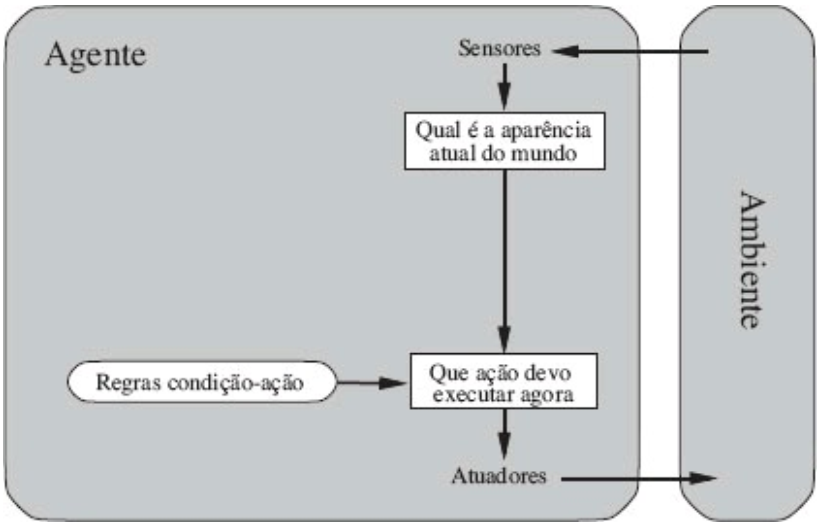
\includegraphics[width=0.9\textwidth]{figuras/figura04}
\end{frame}

\begin{frame}{Agente Reativo Simples}
    \centering
    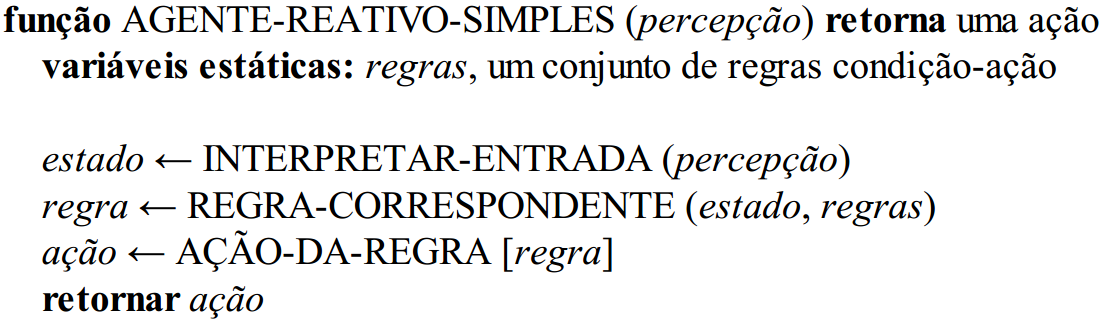
\includegraphics[width=0.9\textwidth]{figuras/figura04_01}
\end{frame}

%- - - - - - - - - - - - - - - - - - - - - - - - - - - - - - - - - - - - - - -
% SUBSUBSECTION 1.3.2
%- - - - - - - - - - - - - - - - - - - - - - - - - - - - - - - - - - - - - - -
\subsubsection{Agente Reativo Baseado em Modelos}

\begin{frame}{Agente Reativo Baseado em Modelos}
    \begin{itemize}
        \justifying
        \item Neste caso, o agente inteligente tem armazenado um modelo de mundo.
    \end{itemize}
    \centering
    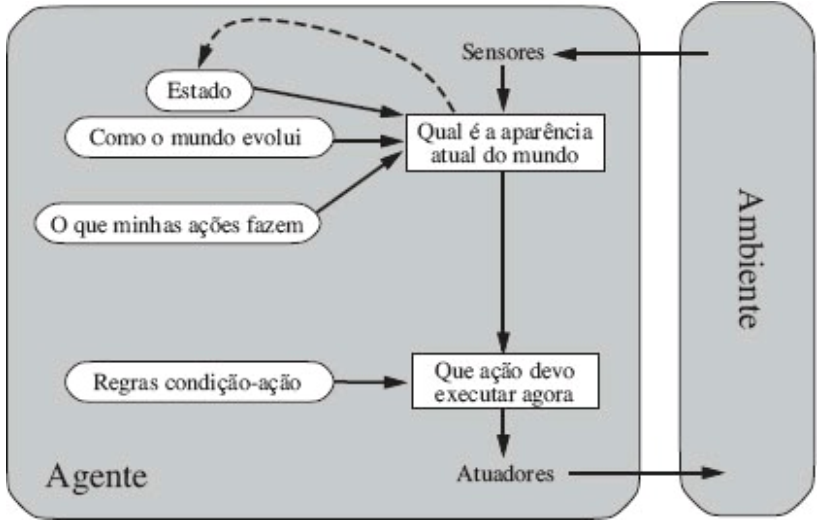
\includegraphics[width=0.9\textwidth]{figuras/figura05}
\end{frame}

\begin{frame}{Agente Reativo Baseado em Modelos}
    \centering
    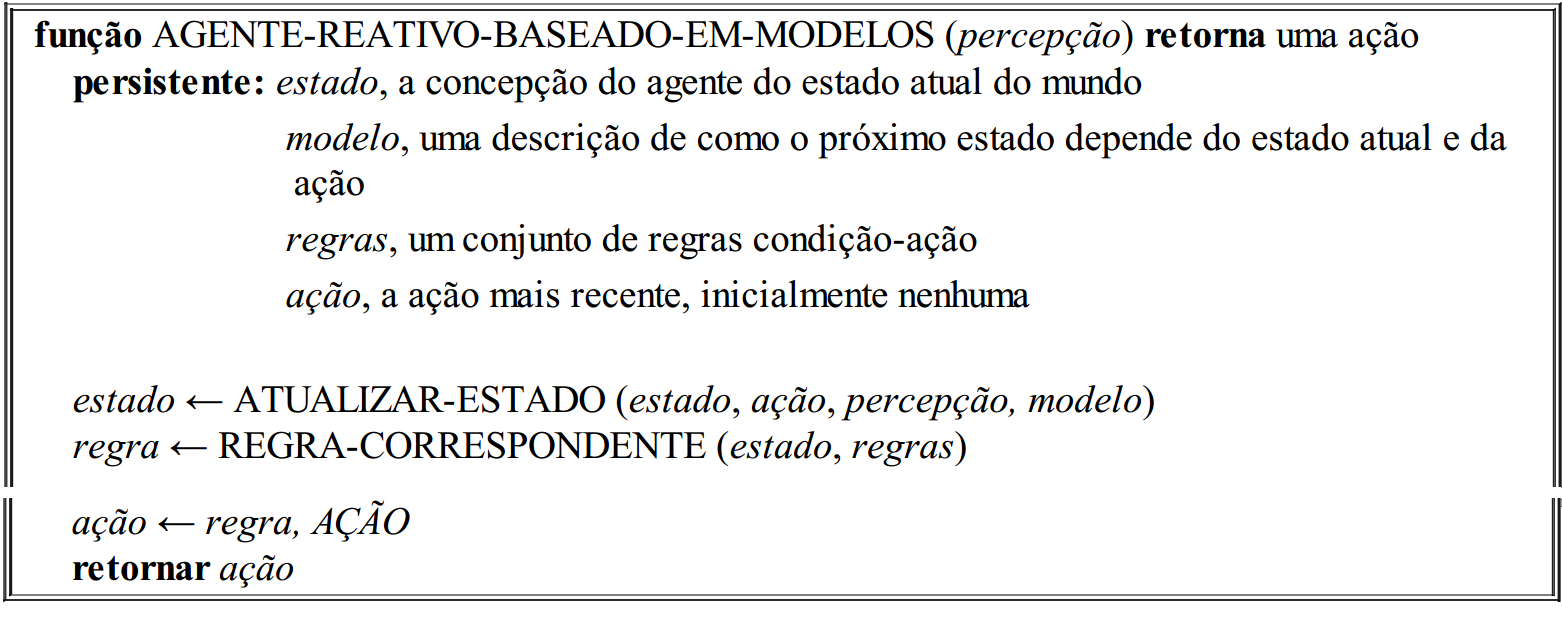
\includegraphics[width=\textwidth]{figuras/figura05_01}
\end{frame}

%- - - - - - - - - - - - - - - - - - - - - - - - - - - - - - - - - - - - - - -
% SUBSUBSECTION 1.3.3
%- - - - - - - - - - - - - - - - - - - - - - - - - - - - - - - - - - - - - - -
\subsubsection{Agente Baseado em Objetivos}

\begin{frame}{Agente Baseado em Objetivos}
    \begin{itemize}
        \justifying
        \item Nem sempre reagir a alguma situação é o suficiente. Muitas vezes o agente precisa de um objetivo para guiar as suas ações.
    \end{itemize}
    \centering
    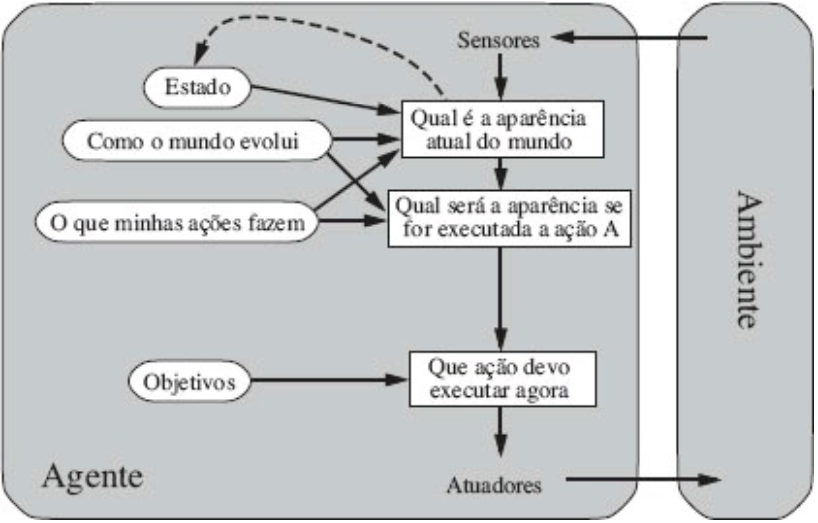
\includegraphics[width=0.9\textwidth]{figuras/figura06}
\end{frame}

\begin{frame}{Agente Baseado em Objetivos}
    \begin{itemize}
        \justifying
        \item Às vezes, a seleção da ação baseada em objetivos é direta --- por exemplo, quando a satisfação do objetivo resulta de imediato de uma única ação. Outras vezes ela será mais complicada --- por exemplo, quando o agente tiver de considerar longas sequências de ações até encontrar um meio de atingir o objetivo.
        \item A partir disso temos duas subáreas da IA: \textbf{Busca} e \textbf{Planejamento}.
    \end{itemize}
\end{frame}

%- - - - - - - - - - - - - - - - - - - - - - - - - - - - - - - - - - - - - - -
% SUBSUBSECTION 1.3.4
%- - - - - - - - - - - - - - - - - - - - - - - - - - - - - - - - - - - - - - -
\subsubsection{Agente Baseado na Utilidade}

\begin{frame}{Agente Baseado na Utilidade}
    \begin{itemize}
        \justifying
        \item Nem sempre os objetivos são suficientes para gerar um comportamento de alta qualidade!
        \item Exemplo: objetivos conflitantes
            \begin{itemize}
                \justifying
                \item<2> Levar um passageiro ao seu destino o mais rápido possível.
                \item<2> Levar um passageiro ao seu destino de forma segura.
            \end{itemize}
        \item<3> Um agente racional baseado em utilidade escolhe a ação que maximiza a utilidade esperada dos resultados da ação, isto é, a utilidade que o agente espera obter, em média, dadas as probabilidades e as utilidades de cada resultado.
    \end{itemize}
\end{frame}

\begin{frame}{Agente Baseado na Utilidade}
    \centering
    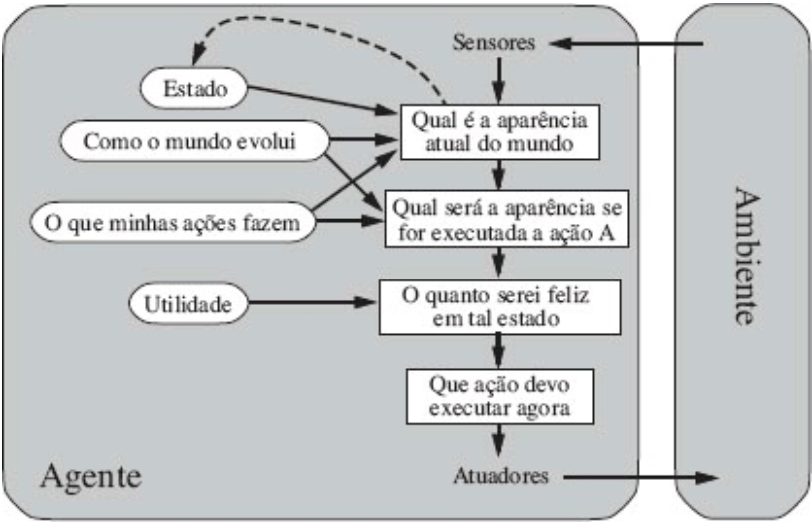
\includegraphics[width=0.9\textwidth]{figuras/figura07}
\end{frame}

%- - - - - - - - - - - - - - - - - - - - - - - - - - - - - - - - - - - - - - -
% SUBSUBSECTION 1.3.5
%- - - - - - - - - - - - - - - - - - - - - - - - - - - - - - - - - - - - - - -
\subsubsection{Agente com Aprendizagem}

\begin{frame}{Agente com Aprendizagem}
    \begin{itemize}
        \justifying
        \item Além de agir de forma racional e inteligente, o agente passa a aperfeiçoar suas ações com o tempo (ou seja, se torna mais competente), mesmo em ambientes inicialmente desconhecidos.
    \end{itemize}
    \centering
    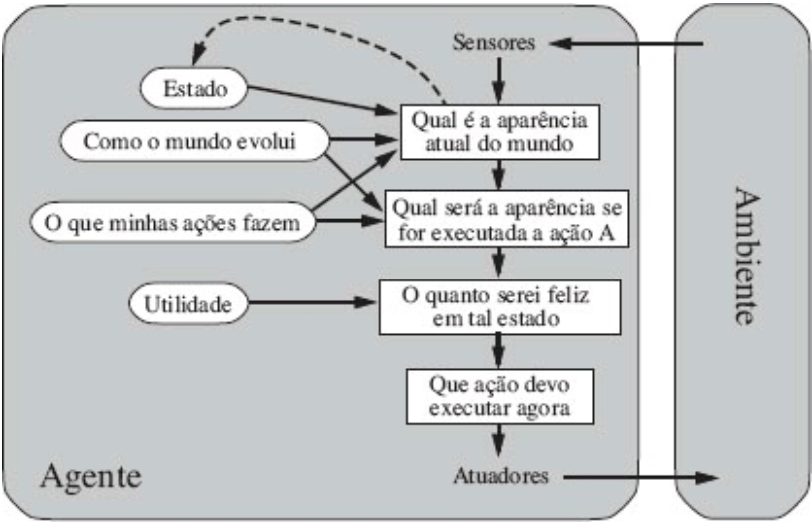
\includegraphics[width=0.9\textwidth]{figuras/figura07}
\end{frame}
%=============================================================================
% SECTION ?
%=============================================================================
\section{FIM}

\begin{frame}{}
    \centering
    \Large
    Terminamos a Segunda Parte!\\
    Obrigado pela atenção!
\end{frame}

%=============================================================================
% SECTION REFERENCES
%=============================================================================
%\begin{frame}[allowframebreaks]{Referências}
%    \scriptsize
%    \printbibliography
%\end{frame}

\end{document}













%% ---------------------------------------------------------------------------
% This presentation is separated by sections and subsections
%\section{Seção I}
%\begin{frame}{Explicações}
%    % itemize
%    Este é um template que pode ser utilizado para:
%    \begin{itemize}
%        \item Apresentação de Trabalhos Acadêmicos
%        \item Apresentação de Disciplinas
%        \item Apresentações de Teses e Dissertações
%    \end{itemize}
%
%    \vspace{0.4cm} % vertical space
%    
%    % enumeration
%    Para utilizar este template corretamente é importante que:
%    \begin{enumerate}
%        \item Tenha conhecimento mínimo sobre LaTeX
%        \item Ler os comentários no template (explicações)
%        \item Ler o README.md (documentação)
%    \end{enumerate}
%
%    \vspace{0.2cm}

%    \example{Este é um texto de exemplo!} \emph{Texto de Ênfase!}
%\end{frame}

%% ---------------------------------------------------------------------------
%\subsection{Subseção I}
%\begin{frame}{Criando Blocos}
%    % Blocks styles
%    \begin{block}{Bloco Padrão}
%        Texto do corpo do bloco.
%    \end{block}

%    \begin{alertblock}{Bloco de Alerta}
%        Texto do corpo do bloco.
%    \end{alertblock}
%
%    \begin{exampleblock}{Bloco de Exemplo}
%        Texto do corpo do bloco.
%    \end{exampleblock}   
%\end{frame}

%% ---------------------------------------------------------------------------
%\subsection{Subseção II}
%\begin{frame}{Criando Caixas}
%    \successbox{testando o success box}
%
%    \pause
%
%    \alertbox{testando o alert box}
%
%    \pause
%
%    \simplebox{testando o simple box}
%\end{frame}

%% ---------------------------------------------------------------------------
%\subsection{Subseção III}
%\begin{frame}{Criando Algoritmos (Pseudocódigo)}
%    \begin{algorithm}[H]
%        \SetAlgoLined
%        \LinesNumbered
%        \SetKwInOut{Input}{input}
%        \SetKwInOut{Output}{output}
%        \Input{x: float, y: float}
%        \Output{r: float}
%        \While{True}{
%          r = x + y\;
%          \eIf{r >= 30}{
%           ``O valor de $r$ é maior ou iqual a 10.''\;
%           break\;
%           }{
%           ``O valor de $r$ = '', r\;
%          }
%         } 
%         \caption{Algorithm Example}
%    \end{algorithm}
%\end{frame}

%% ---------------------------------------------------------------------------

%\begin{frame}{Inserindo Algoritmos}
%    \lstset{language=Python}
%    \lstinputlisting[language=Python]{code/main.py}
%\end{frame}

%% ---------------------------------------------------------------------------
%\begin{frame}{Inserindo Algoritmos}
%    \lstinputlisting[language=C]{code/source.c}
%\end{frame}

%% ---------------------------------------------------------------------------
%\begin{frame}{Inserindo Algoritmos}
%    \lstinputlisting[language=Java]{code/helloworld.java}
%\end{frame}

%% ---------------------------------------------------------------------------
%\begin{frame}{Inserindo Algoritmos}
%    \lstinputlisting[language=HTML]{code/index.html}
%\end{frame}

%% ---------------------------------------------------------------------------
% This frame show an example to insert multicolumns
%\section{Multicolunas}
%\begin{frame}{Seção II - Multicolunas}
%    \begin{columns}{}
%        \begin{column}{0.5\textwidth}
%            \justify
%            É possível colocar mais de uma coluna utilizando os comandos de $\backslash$begin\{column\}\{\} e $\backslash$end\{column\}
%        \end{column}
%        \begin{column}{0.5\textwidth}
%            \justify
%            Porém, o espaçamento deve ser proporcional entre as colunas para que estas colunas não entrem em coflito. O espaçamento é dado pelo segundo argumento do $\backslash$begin.
%        \end{column}
%    \end{columns}    
%\end{frame}

%% ---------------------------------------------------------------------------
% This frame show an example to insert figures
%\section{Imagens}
%\begin{frame}{Seção III - Figures}
%    \begin{figure}
%        \centering
%        \caption{Emblema da UFC.}
%        
\includegraphics[scale=0.3]{libs/emblemufc.pdf}
%        \source{Obtido pelo site oficial da UFC \cite{siteufc} \cite{einstein}}
%        \label{fig:ufc_emblem}
%    \end{figure}
%\end{frame}

%% ---------------------------------------------------------------------------
% Reference frames
%\begin{frame}[allowframebreaks]
%    \frametitle{Referências}
%    \printbibliography
%\end{frame}

%% ---------------------------------------------------------------------------
% Final frame
%\begin{frame}{}
%    \centering
%    \huge{\textbf{\example{Obrigado(a) pela Atenção!}}}
%    
%    \vspace{1cm}
%    
%    \Large{\textbf{Contato:}}
%    \newline
%    \vspace*{0.5cm}
%    \large{\email{usuario@dominio}}
%\end{frame}